\documentclass[UTF8]{ctexart}
\usepackage{amsmath}
\usepackage{multirow}
\usepackage{float}
\usepackage{graphicx}
\usepackage{geometry}
\usepackage{diagbox}
\usepackage{hyperref}

\pagestyle{plain}
\geometry{a4paper,total={170mm,257mm},left=20mm,top=20mm}
\title{\heiti \zihao {-2} 可交互式钟表页面说明文档}
\author{组长:白润声 2021011793 \\ 组员:王皓雯 2021011815、林敏芝 2021011791、郭嘉伟 2021011787}
\date{}

\CTEXsetup[name={第,部分}]{section}
\CTEXsetup[format={\zihao{-3}\raggedright\bfseries}]{section}
\geometry{a4paper,left=20mm,right=20mm}

\begin{document}
	\maketitle
	\section{实现结果}
	
	\begin{figure}[!htb]
		\centering
		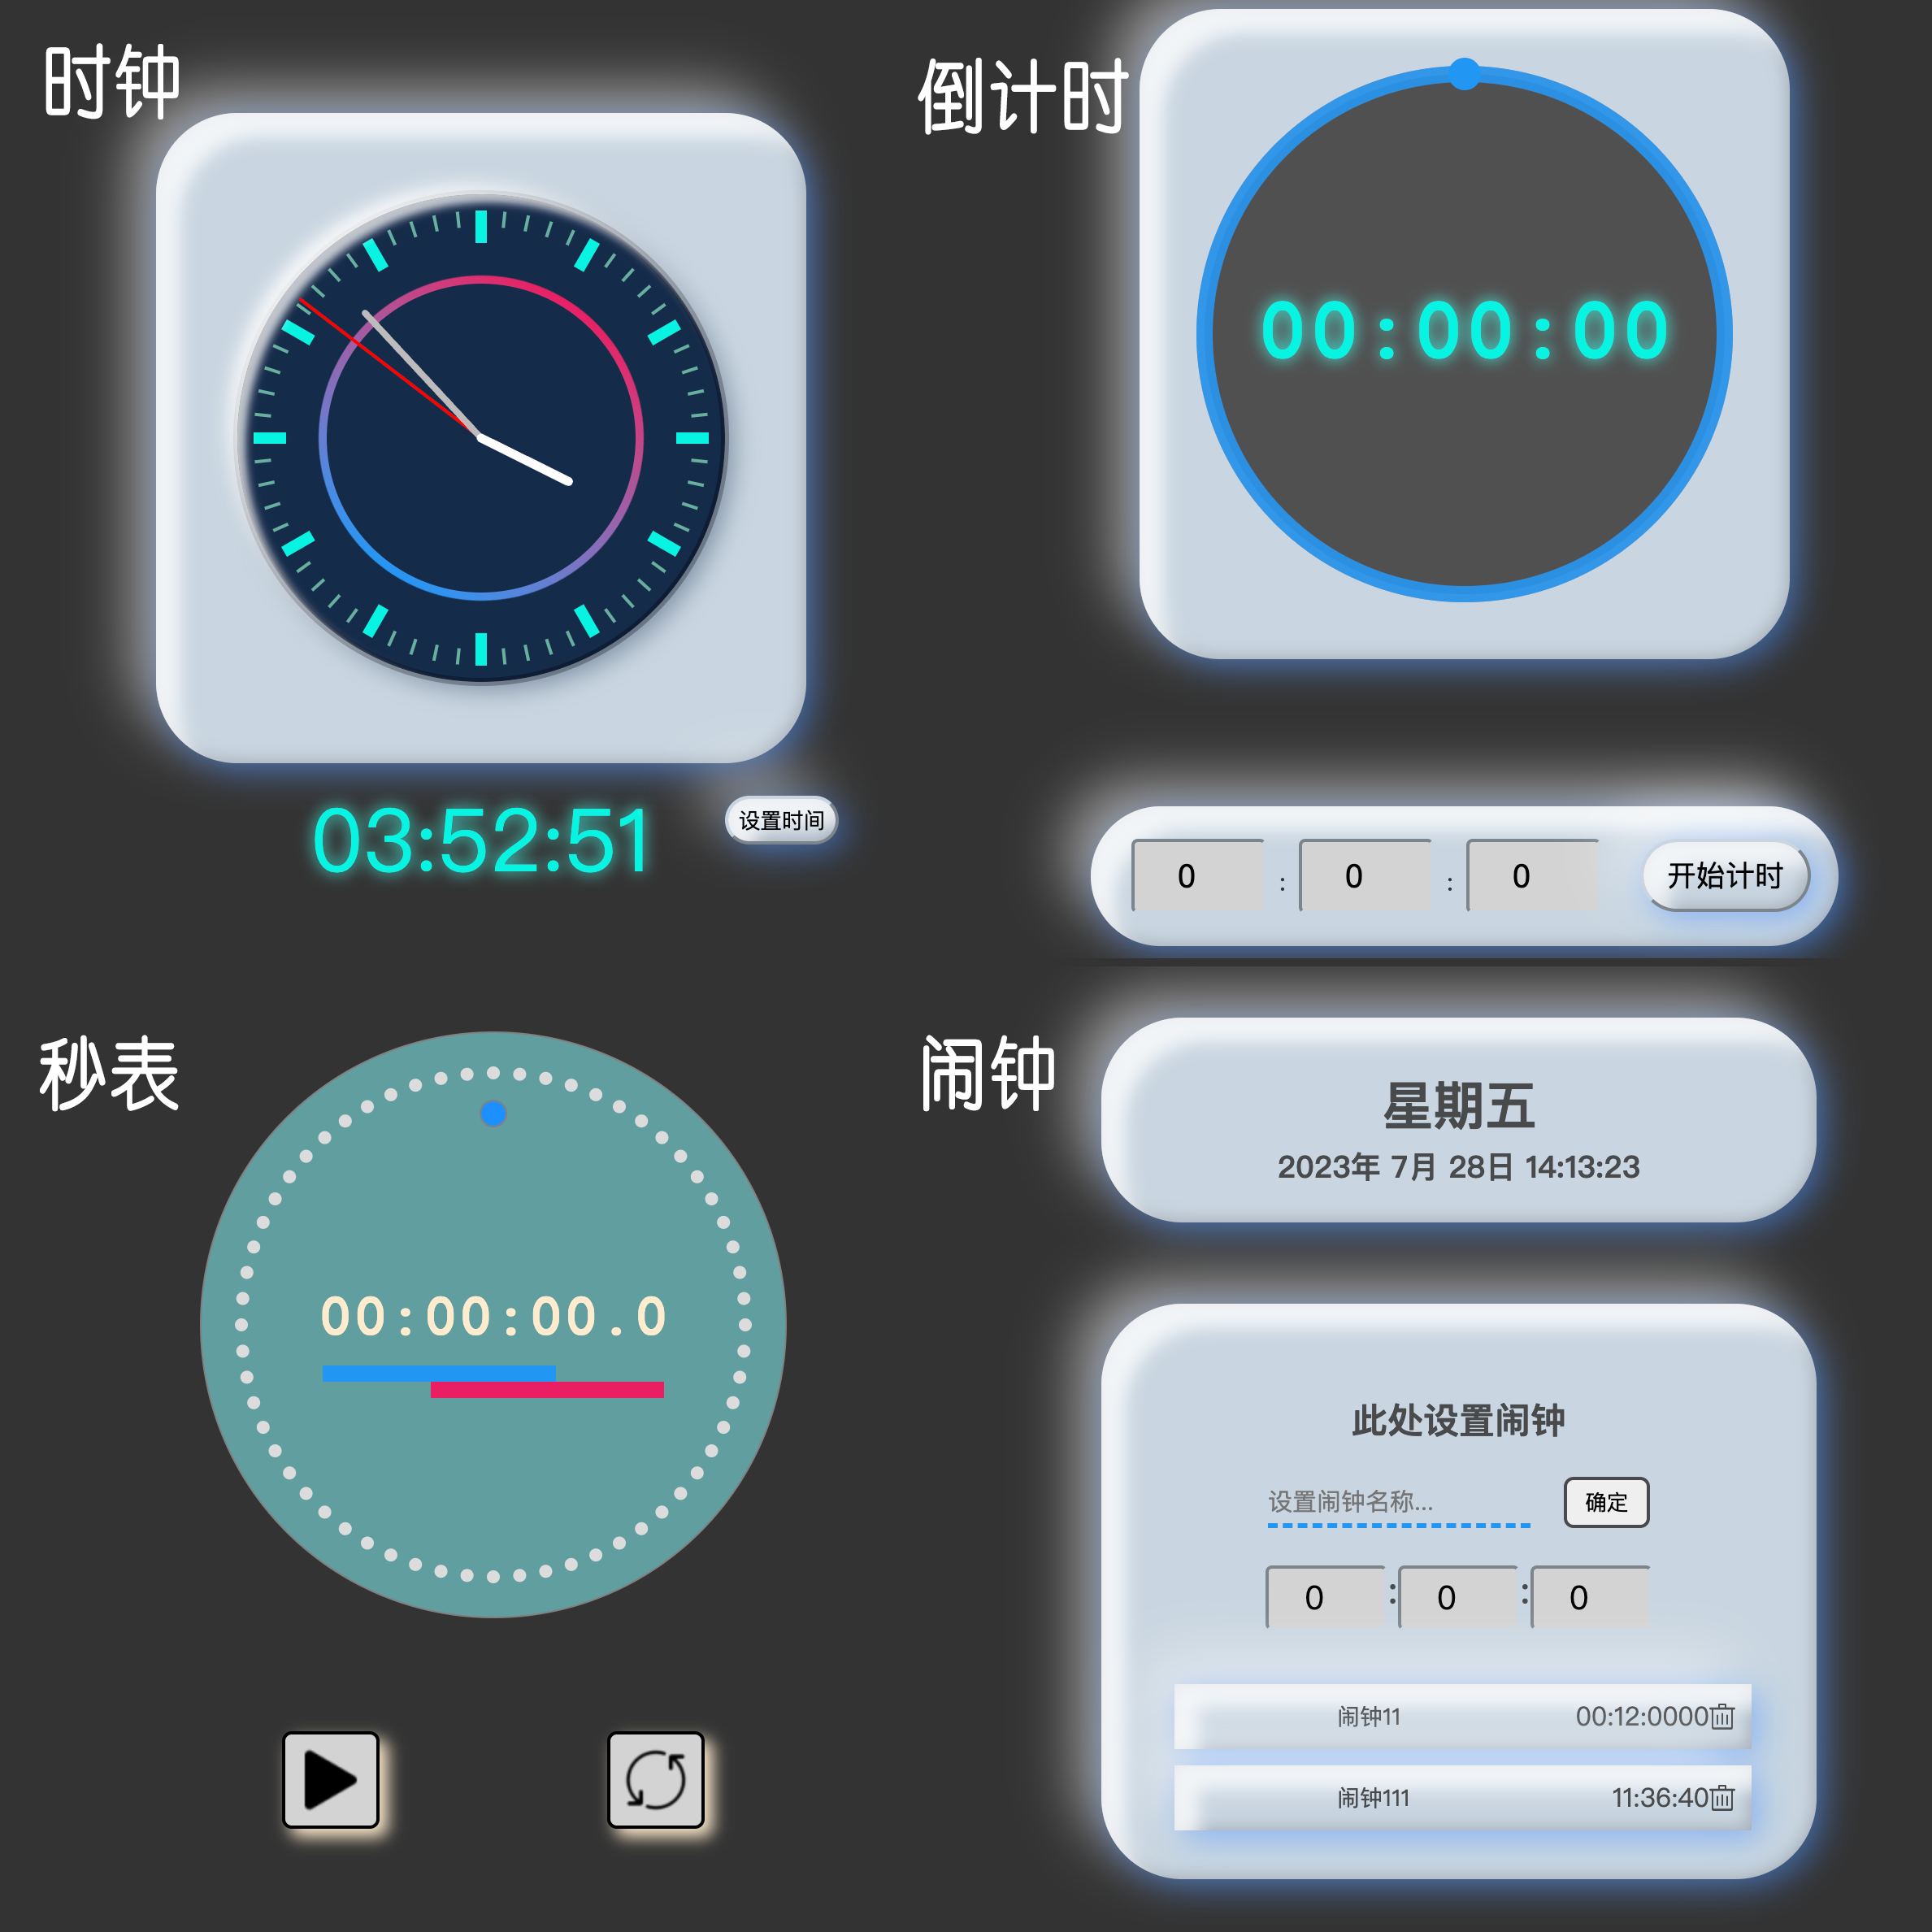
\includegraphics[width=\linewidth]{总体展示图.png}
		\caption{四种模式简单展示}
	\end{figure}
	
	\section{实现思路} % 简要阐释功能点的实现思路
	% 以下是各功能点,大家可以简要解释自己负责部分的思路。文字写在每个\paragraph下的空行即可。
	\paragraph{逻辑架构}
	 我们将时间离散化,每秒分为20tick,因此一个时刻对应(hour, minute, second, tick)。在此基础上我们实现了clock类,该类是所有表的逻辑架构,内部元素包含确定时刻的四个值,同时支持以下接口:1.获取时/分/秒针角度;2.获取时间字符串;3.获取与设置总tick数;3.设置时/分/秒/tick;4.tick自增与自减。每个不同的表都由一个clock类控制。
	\paragraph{页面切换}
	在main页面上方绘制菜单栏,菜单栏的光标会随着鼠标悬停的位置改变位置和颜色。当鼠标单击对应页面的标志时,就在下方的container中放入对应页面。点击时,先依据滑动的方向将container的位置放置到左侧或者右侧,再令其滑动至画面中央,从而实现滑动切换的视觉效果。
	\paragraph{钟表}
	表盘的核心部分在于时钟运行动画的设置,而控制动画的核心逻辑是Clock类。实例化一个Clock对象clock,将clock当前时间设置为想要的时间,之后可以通过clock中tick的自增来模拟时间的流逝。依照我们的设计,clock每次自增1tick,对应时间50ms,那么我们只需要调用setInterval函数,将时间间隔设置为50ms,然后在到时响应函数中进行tick的自增,同时获取当前clock中时针、分针、秒针的相应角度。有了三个角度作为参数,调用用来与页面显示打交道的drawClock()接口,就能实现表盘的绘制。
	
	drawClcok()接口中分别对时针、分针、秒针的位置进行设置。由于三个针都是用svg的Line绘制的,所以只需要设置其行走端的(x,y)坐标即可,具体设置方法就是几何上的一些操作。
	
	\paragraph{表针拖动}
	表针拖动功能的实现主要依靠表针对象对鼠标事件的监听。当鼠标拖动时,首先记录当前时间,之后算出鼠标移动的角度。根据不同的表针,算出不同的时间增量,再对钟表的时间进行更新。通过时间的更新,实现表针位置的自动更新。
	
	\paragraph{计时器}
	表盘绘制:利用svg技术,画出圆盘背景,指针点和标记点。表盘中动画由红、蓝两道条纹进行不断循环的animation实现。
	运行:基于clock类实现。利用setTimeInteval,每50ms控制clock自增,并获取秒针角度更新指针点、获取时间字符串以更新现实中。
	\paragraph{秒表}
	表盘绘制:利用svg技术,画出背景板,计时凹槽、环和点。
	运行:基于clock类实现。在时间设置区获取到时间后首先设置clock时间,记录总tick数。其后setTimeInteval,每50ms控制clock自减,通过剩余总tick计算剩余比例以设置计时环和点。页面下方的设置时间区和按钮区为两大小、位置相同的区域,交替设置visible、hidden以实现切换效果。
	\paragraph{闹钟}
	绘制:利用css绘制世界时间,利用svg技术显示已设置成功的闹钟列表。通过在javascript中对列表进行更改来动态更新,在每次闹钟被改变之后都会重新渲染。闹钟机制的实现方法是每一秒都比较当前时间和闹钟的设置时间是否相同,若相同则弹出提示并播放闹铃。
	
	% -------------------- 分界线 -------------------- %
	
	\section{使用说明及交互方式} % 简要说明各部分的使用方法
	\paragraph{整体页面}
	在html目录下,点击main.html即可进入使用。整体页面包括导航栏与主体页面。导航栏由4个图标与1个marker组成。4个图标对应的功能分别为钟表、计时器、秒表和闹钟。当鼠标悬浮或点击图标时,对应的图标会亮起,并且marker会平滑地移至图标后侧,同时呈现出不同色彩。点击不同图标,页面会平滑地进行切换。
	\paragraph{钟表}
	拖动钟表的表针即可实时改变钟表的时间。点击“设置时间”按钮也可进行时间修改。请注意输入的时间必须合法。
	\paragraph{计时器}
	左下侧为开始/暂停按钮,右下侧为重置按钮。点击开始按钮,计时器开始运行,其后切换为暂停按钮,再次点击则计时器暂停。重置按钮仅在暂停时可用,点击后会将时间设置为00:00:00。
	\paragraph{秒表}
	在时、分、秒框中输入时间后,若输入合法则会开始计时,且输入框切换为控制按钮。控制按钮依次为开始/暂停按钮、重置按钮和取消按钮。其中重置按钮点击后会重新将时间恢复为最初设置时间而,取消按钮点击后则会清除当前计时并切换回输入框。
	\paragraph{闹钟}
	在时、分、秒框中输入时间并在闹钟名称部分输入闹钟名后,若输入合法且闹钟名称不为空则设置闹钟成功,会在输入区下方累计显示闹钟的名称和时间,并分别显示每个闹钟的删除按钮,单击删除按钮可以删除对应闹钟。当时间达到闹钟设置的时间时,就会弹出到了闹钟时间的提示,并播放闹铃。
	

	\section{遇到问题及解决方法}% 这个大家也得多少写点,要求里有
	\subsection{倒计时进度条在时间归零时有残留}
	在制作倒计时的环状进度条时,出现了一个问题:当时间归零时弹出提示框,但此时环状进度条还有一点点没有走完(但实际上时间已经归零了),但是点掉提示框后进度条就归零了。这与想要的效果不符,更奇怪的是与逻辑也不符,即为什么时间都到零了,按照时间画的进度条还能不到零。解决:后来经过反复研究发现,原来javascript中alert()弹窗提示这个方法是一种阻断式函数调用,即alert被调用后会阻断后续的函数调用,知道提示框被点掉。于是,我们想到可以为alert用setTimeout设置一个延迟调用,使得alert异步进行,防止alert阻断绘制事件的发生。结果bug解决。
	
	
	\section{参考资料} % 如果有的话就写一下
	JS + HTML + CSS 实现Todolist-CSDN博客: \url{https://blog.csdn.net/Wksycxy/article/details/127792977?ops_request_misc=&request_id=&biz_id=102&utm_term=todolist}

	
	【教程演示】2021最具创意的16个CSS特效:\url{https://www.bilibili.com/video/BV1nT4y1977i?p=2&vd_source=873c347266938fb6766020bedd9fb369}
	
	JS实现前端组件环形的SVG进度条:\url{https://www.swvq.com/article/detail/977/}

\end{document}